\documentclass[a4paper]{article}

\usepackage[utf8]{inputenc}

\usepackage{url}
\usepackage[]{hyperref}

\usepackage{caption}

\usepackage{listings}

\usepackage{color}

% *** GRAPHICS RELATED PACKAGES ***
%\usepackage[pdftex]{graphicx}
\usepackage{graphicx}
%\usepackage[dvips]{graphicx}
% to place figures on a fixed position
\usepackage{float}

\usepackage{tabularx}

\usepackage{nth}

\usepackage[margin=1in]{geometry}

\title{Docker - syllabus}
\author{}
\date{}


\begin{document}

\maketitle

\tableofcontents

\section{Linux containers}
The Linux Containers (LXC) provide operating system level virtualized environment in which isolated Linux systems
(containers) can be run on the Linux host machine. The operating system level environment virtualization can be viewed
as lightweight Virtual Machines (VMs). What makes this better compared to VMs? It requires less disk space compared
to a fully virtualized guest OS, provides rapid creation and fast operation. In contrast to emulating the full hardware
environment Containers use a shared, common OS kernel resulting in more efficient runtime performance compared to
full-fledged OS virtualization.

In another aspect it is called ``chroot on streoids". The \emph{chroot} utility runs the specified command or
interactive shell using the root directory specified as command argument. The process run by chroot is quasi ``locked"
inside the specified directory, it can not reach any of the files outside that. This can be used for creating a system
within the system.

\begin{figure}[H]
    \centering
    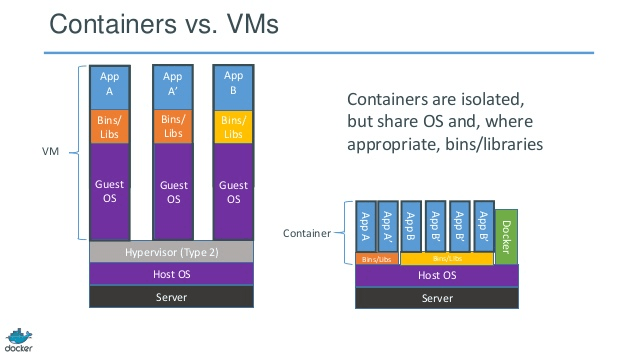
\includegraphics[width=0.9\textwidth]{figures/container_vs_vm.png}
    \caption{Containers vs. VMs}
    \label{fig:containers}
\end{figure}

The Linux kernel's control groups (\emph{cgroups}) function provides facilities for partitioning and prioritizing
resources without having to
start virtual machines. Furthermore with the help of \emph{namespaces} the visibility of file systems, user IDs,
network connections can be
isolated for individual applications. As a result a unique runtime environment can be created for the application that
runs isolated from
the other containers and from the host machine.
The container application's dependencies (software suites, libraries, configuration files) can be embedded into the
container resulting in
a highly portable, restartable, manageable unit.
For example one can create a container for a web server, another one for its database, yet another one for their message
queue or alternatively these
can be combined into a single container hence allowing the creation of modular application architecture.
If a user packs his self-developed software into a container it can be ensured that the software will be able to
execute on another host machine regardless from the type of the host (developer machine, user machine, application
server etc.) resulting in great flexibility in terms of portability.
If an executable can be executed on a Linux box that executable can packed into a Linux Container also. Containers provide a new
and easier way of working in application coding, building, installation and execution and can be installed easily on
machines running in a cloud provider's environment.

\section{Docker}

Docker offers an open-source platform for managing containers that can be used for development and execution of
distributed applications
while maintaining portability.
It provides a common toolset for programmers, development teams and for operations personnel (DevOps) that can
exploit the benefits
of distributed network applications.
The Docker runtime runs as a daemon in the background managing the containers, the images and the creation of those.

The goal of Docker is to simplify the usage of LXC and beside that it allows the containers to be used on different
types of Linux
distributions -- i.e. it abstracts the LXC system specific parts. In the beginning Docker used the LXC format but
currently it uses its own
container format. One important difference between those two formats is that in LXC there is an \emph{init} process as
a consequence multiple
processen can be run in parallel inside a container. In contrast Docker format doesn't have one so only one process can be run. (For detailed list of
differences please see \url{https://www.flockport.com/lxc-vs-docker/})

Docker's architecture follows the client-server based model as illustrated on Figure~\ref{fig:arch}. The commands
requested by the Docker client are executed by the Docker daemon (engine, server).
The user has no direct interaction with the Docker daemon only through the Docker client -- this is the ``docker" utility --
that provides the
user interface. The client and the daemon can run on the same machine or the client can connect to a remote daemon
process alternatively. The communication can be carried out either over sockets or over RESTful API.

\begin{figure}[H]
    \centering
    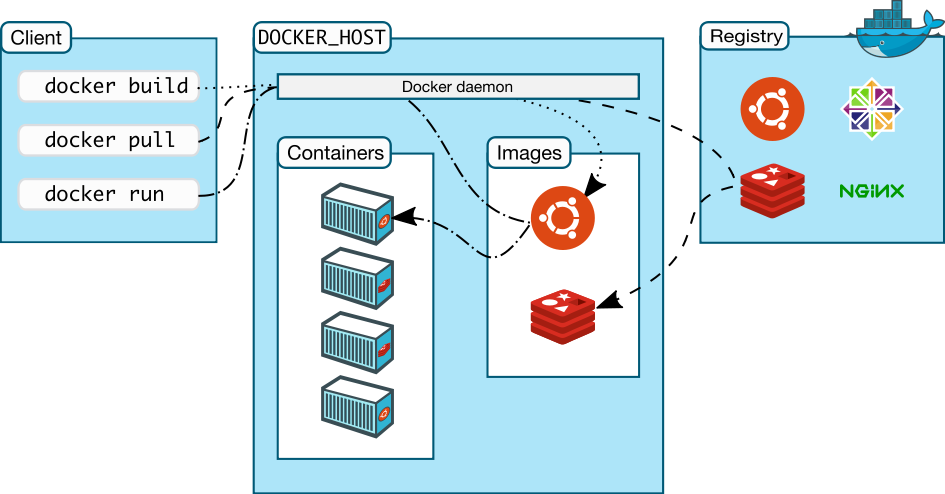
\includegraphics[width=0.9\textwidth]{figures/docker_arch.png}
    \caption{Docker components and architecture}
    \label{fig:arch}
\end{figure}

Docker requires an image file from a given operating system. The image is a write-protected template that is used for
starting the containers.
When running the container this is augmented with an upper layer of writeable filesystem that is used for running the
application. The image file
is basically a pre-installed system that is composed from \emph{aufs} or \emph{btrfs} layers (Union File System) and it
is version controlled as it can be seen on Figure~\ref{fig:layers}.
At startup there is a base image -- e.g. Ubuntu or Debian -- and  all the overlaying file-systems are joined
together to form a final file-system. Additional layers can be placed on any image -- not just the base image -- to
modify that for certain needs. The image files can be created by the user or downloaded from Docker Hub web-page
created by other users. Docker Hub is a public repository but a privately hosted repository can also be used. The
custom made images can be uploaded and shared with the community.

\begin{figure}[H]
    \centering
    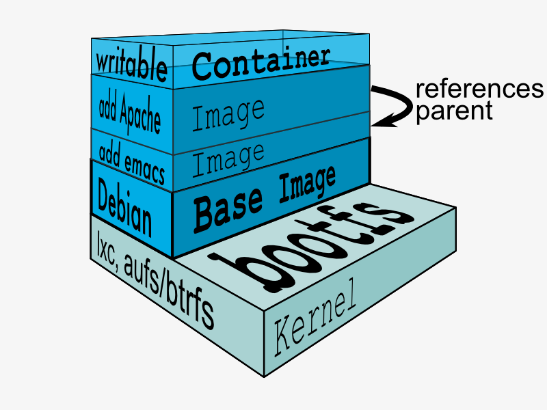
\includegraphics[width=0.9\textwidth]{figures/docker_layers.png}
    \caption{Docker layers}
    \label{fig:layers}
\end{figure}

A container is actually a running entity of a given image. Multiple containers can also be run from the same image file
simultaneously.

Creation and extension of Docker image files can be done in two ways: either by entering into the container manually
and installing and configuring the desired software then by saving the resulting image file or by using a
\emph{Dockerfile} that has a script-like syntax where the
installable components can be declared easily.

\section{Further Reading}

\begin{itemize}
    \item Docker overview: \url{https://docs.docker.com/engine/docker-overview/}
    \item Docker introduction: \url{https://docs.docker.com/get-started/} Part 1. and 2.!
\end{itemize}

\appendix

\section{Entry quiz sample questions}

\begin{enumerate}
    \item What is the difference between the VMs and the Linux Containers?
    \item Which Linux kernel functions allow the implementation of containers?
    \item What is the relation between Docker images and containers?
    \item How are Docker images used, who can create them, how can one obtain them?
    \item How are Docker images extended/updated?
    \item What are the purposes of interactive and daemon modes?
    \item What is the difference between docker run and docker start commands?
    \item How are the container network interfaces mapped to the host machine?
\end{enumerate}

\section{Lab exercises}

\subsection{Lab environment \& introduction}

The task is to implement a sample application (web server + database) using containers. The code of the index page of
the web server is a simple PHP application that saves the time of the first visit into the database and the count of
visits since then and also displays those in the resulting HTML.

\subsubsection{Preparations}
\begin{itemize}

    \item Boot menu: P2P+SDN under SPRING (TC 5.2 64bit + VBOX)

    \item Docker engine simple installation: \emph{curl -sSL https://get.docker.com/ | sh}

    \item \textbf{If the docker engine has not been started automatically execute: \emph{sudo service docker start}}

\end{itemize}

\textbf{All docker commands have to be executed using root privileges!}

The missing applications can be installed in the containers on demand (e.g. mysql, ab, etc.)

During the exercises an arbitrarily chosen image file can be used. The instructions below are based on a concrete
`apache + mysql' image.

\subsubsection{List of important commands}
\begin{table}[h]
    \begin{tabularx}{\textwidth}{|l|X|}
        \hline docker ps                                                                     & list of running containers                       \\
        \hline docker ps -a                                                                  & list of all containers seen by the docker daemon \\
        \hline docker images                                                                 & list of the locally available image files        \\
        \hline docker inspect \textless~container\textgreater or \textless~image\textgreater & detailed information on the
        give container/image file                                                                                                               \\
        \hline docker run -d \textless~image\textgreater \textless~command\textgreater       & create and start a new container
        based on the given image file running the command specified (runs in the background because of -d)                                      \\
        \hline docker start/stop \textless~container\textgreater                             & start/stop an existing container                 \\
        \hline docker exec -it \textless~container\textgreater bash                          & open a new bash shell to the running container   \\
        \hline docker rm -f \textless~container\textgreater                                  & delete container, even if it's running           \\
        \hline
    \end{tabularx}
\end{table}

\subsection{Task 1.}

Implement the two application components in two separate containers. (By default one Docker container can run one
process)
You can use already existing image files. For starters read through the corresponding reference with examples
\url{https://docs.docker.com/engine/reference/commandline/images/}

\subsubsection{Application containers}
The description of the image files can help on the usage of them. For example in case of \emph{mysql}: how to set the
root password, how to set-up the data volume etc.

\textbf{\emph{\nth{1} container}}: the web-server container is apache with PHP e.g.: \url{https://hub.docker.com/_/php/}

For the apache support a suitably tagged image file has to be used! For the php mysqli support  version 7 has to
be used: php:7-apache

By default in this image php mysqli is not installed. To add it a new Dockerfile has to be created and an image has to
be built. (see details on the image web page under ``How to install more PHP extensions" section). In this sample
exercise the extension to be used is : mysqli

The resulting Dockerfile has to be documented in the lab report!

Help:
\begin{itemize}
    \item \url{https://docs.docker.com/get-started/part2/#define-a-container-with-a-dockerfile}
    \item \url{https://docs.docker.com/get-started/part2/#build-the-app}
\end{itemize}

\textbf{\emph{\nth{2} container}}: database container with MySQL: \url{https://hub.docker.com/_/mysql/}

\subsubsection{Interconnecting two containers}
Create a new inter-container virtual network and connect the previous containers to it:
\url{https://docs.docker.com/engine/tutorials/networkingcontainers/#create-your-own-bridge-network}

Document in the lab report that which commands were used creating the network, for starting the containers and the
proof that the containers can reach each other on IP level (ping utility)

\subsubsection{Web content and database upload}

For both storing the html/php pages and for the database data use the data volume attached to the host machine (bind
mount data volume): \url{https://docs.docker.com/engine/admin/volumes/bind-mounts/}

Document  in the lab report the docker commands used!

Expected result: the web content will be available on the volume mounted to the host machine as a result it can be
edited on the host machine while the container is running.

\textbf{\emph{\nth{1}}}: The following database will be needed for storing the statistics about the web page visits:

Database name: log

Table name: pagestats

scheme:  url (varchar[80]) primary key, hits (int), since (timestamp)

For creating the mysql database in the database container the \emph{create\_sql.txt} script can be used:
\begin{lstlisting}[language=bash,breaklines]
mysql -h [host] -u [user] -p < create_sql.txt
\end{lstlisting}

How is the database accessed from the host machine? What ports are reachable on the container? (commands + answer must
go into the report)

\textbf{\emph{\nth{2}}}:  Modify the php file found
here:\url{https://qosip.tmit.bme.hu/foswiki/pub/Meres/DockerFeladatok/index.php.txt} so that it can connect to the
database. The resulting php file has to be documented!

How is the database accessed from the web container (from the php file)?

Check and document the operation of the web page!

What happens to the counter if the container is deleted and started again with the same arguments?

\subsection{Task 2.}
Running the two application components from a single container. (By default only one process can be run in a container)

Inside one container using image e.g. linuxconfig/lamp, description
\url{http://linuxconfig.org/lamp-linux-apache-mariadb-php-stack-docker-image-deployment}

In this image the web directory can be mounted as data volume but this image is not prepared for mounting the database
directory. Try and mount the database directory as a data volume similarly as in the previous task. What do we see in
the docker logs?

Which ports are reachable on the container?

Since the default config does not allow to connect to the DB running in the container using mysql client then log in to
the container (docker exec) and create the database and scheme required for the page stats application from there using
the mysql client manually by executing the commands from the create\_sql.txt script.

Create the web content. What has to be modified in the PHP file compared to the previous solution? (How the database is
accessed?)

By default one Docker container can run only one process. If running multiple processes is desired then the use of a
process management device is required e.g. supervisord.
\url{https://docs.docker.com/engine/articles/using_supervisord/}

Check and understand how the supervisord is configured in the container 
(/etc/supervisor/conf.d/supervisord.conf)

Create a Dockerfile that allows ssh login into the container. Help can be found
here:\url{https://docs.docker.com/engine/examples/running_ssh_service/} Modify the specified Dockerfile statements if
required! (e.g. /etc/ssh/sshd\_config)

Check and document the operation of the webpage!

What happens to the counter if the container is deleted and started again with the same arguments?

Check and document that the ssh access is working!

\subsection{Task 3.}

Benchmark both application's performance using the apache bench utility (\emph{ab}). For example \emph{`ab -n 100 -c 10
    \textless~URL\textgreater}

\end{document}